\documentclass{article}

% Language setting
% Replace `english' with e.g. `spanish' to change the document language
\usepackage[english]{babel}

% Set page size and margins
% Replace `letterpaper' with`a4paper' for UK/EU standard size
\usepackage[a4paper,top=2cm,bottom=2cm,left=3cm,right=3cm,marginparwidth=1.75cm]{geometry}

% Useful packages
\usepackage{amsmath}
\usepackage{graphicx}
\usepackage{listings}
\usepackage{xcolor}
\usepackage[colorlinks=true, allcolors=blue]{hyperref}

\definecolor{codegreen}{rgb}{0,0.6,0}
\definecolor{codegray}{rgb}{0.5,0.5,0.5}
\definecolor{codepurple}{rgb}{0.58,0,0.82}
\definecolor{backcolour}{rgb}{0.95,0.95,0.92}

\lstdefinestyle{mystyle}{
    backgroundcolor=\color{backcolour},   
    commentstyle=\color{codegreen},
    keywordstyle=\color{magenta},
    numberstyle=\tiny\color{codegray},
    stringstyle=\color{codepurple},
    basicstyle=\ttfamily\footnotesize,
    breakatwhitespace=false,         
    breaklines=true,                 
    captionpos=b,                    
    keepspaces=true,                 
    numbers=left,                    
    numbersep=5pt,                  
    showspaces=false,                
    showstringspaces=false,
    showtabs=false,                  
    tabsize=2
}

\lstset{style=mystyle}

\title{Homework 3\\CS3316 Reinforce learning}
\author{Ng Tze Kean\\Student number: 721370290002}

\begin{document}
\maketitle

\begin{titlepage}
\end{titlepage}

\section*{Architecture}

We design the program to take in the gridworld but with a cliff. This time the
starting position is fixed, and the agent has to navigate to the goal state on
the opposite end of the map.

\begin{figure}[h]
    \centering
    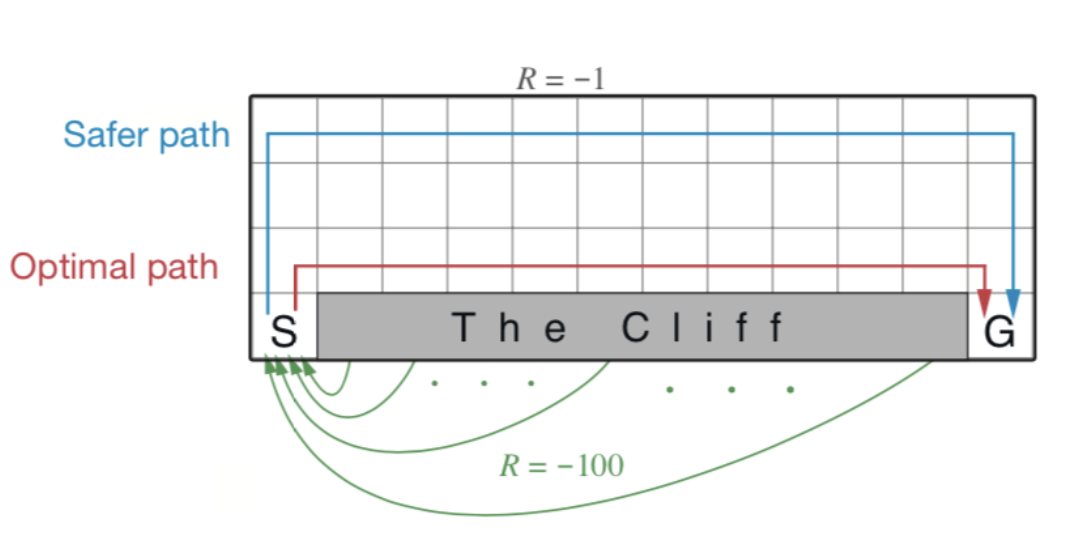
\includegraphics[width=0.7\textwidth]{image.png}
\end{figure}

The agent can take multiple paths to the goal state as shown in the image. If
the agent however, steps into the cliff, he will fall and return to the start
point and receive a reward of -100. Ideally, the agent will take the path closest
to the cliff to the goal, to minimize the negative rewards that he receives. We
will see in the following 2 algorithm how the model performs and what we can infer
from the learning.

\section*{SARSA}

\begin{figure}[h]
    \centering
    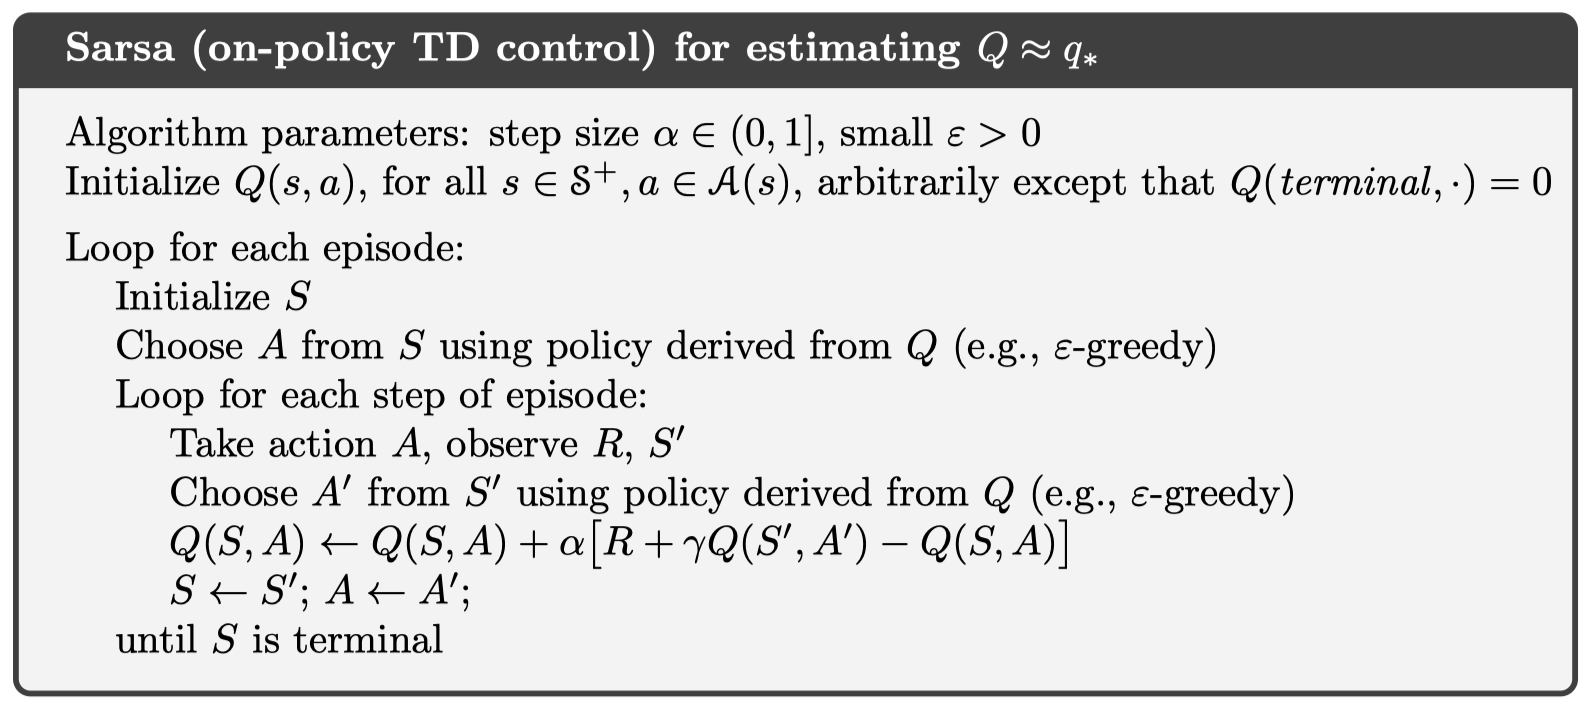
\includegraphics[width=0.7\textwidth]{image-1.png}
\end{figure}

From SARSA, we can see that the agent is learning on policy. This means that the
agent is learning the value of the policy that it is currently following. This
is done by looking at the next state and the action that the agent will take in
the next state. The agent will then update the quality of the current state and
action based on the reward it receives and the quality of the next state and
action.

\begin{lstlisting}[language=Python, caption=SARSA code]
s = self.grid.state
action = self.get_action()
steps = 0
while not self.grid.is_finish() and steps < self.run_limit:
    s_prime, reward = self.grid.next_step_and_reward(action)
    # on policy learning
    action_prime = self.get_action()
    self.quality[(s,action)] += \
            self.alpha * (
                reward + \
                self.gamma * self.quality[(s_prime,action_prime)]\
                - self.quality[(s,action)]
            )
    action = action_prime
    s = s_prime
\end{lstlisting}

\section*{Q Learning}

\begin{figure}[h]
    \centering
    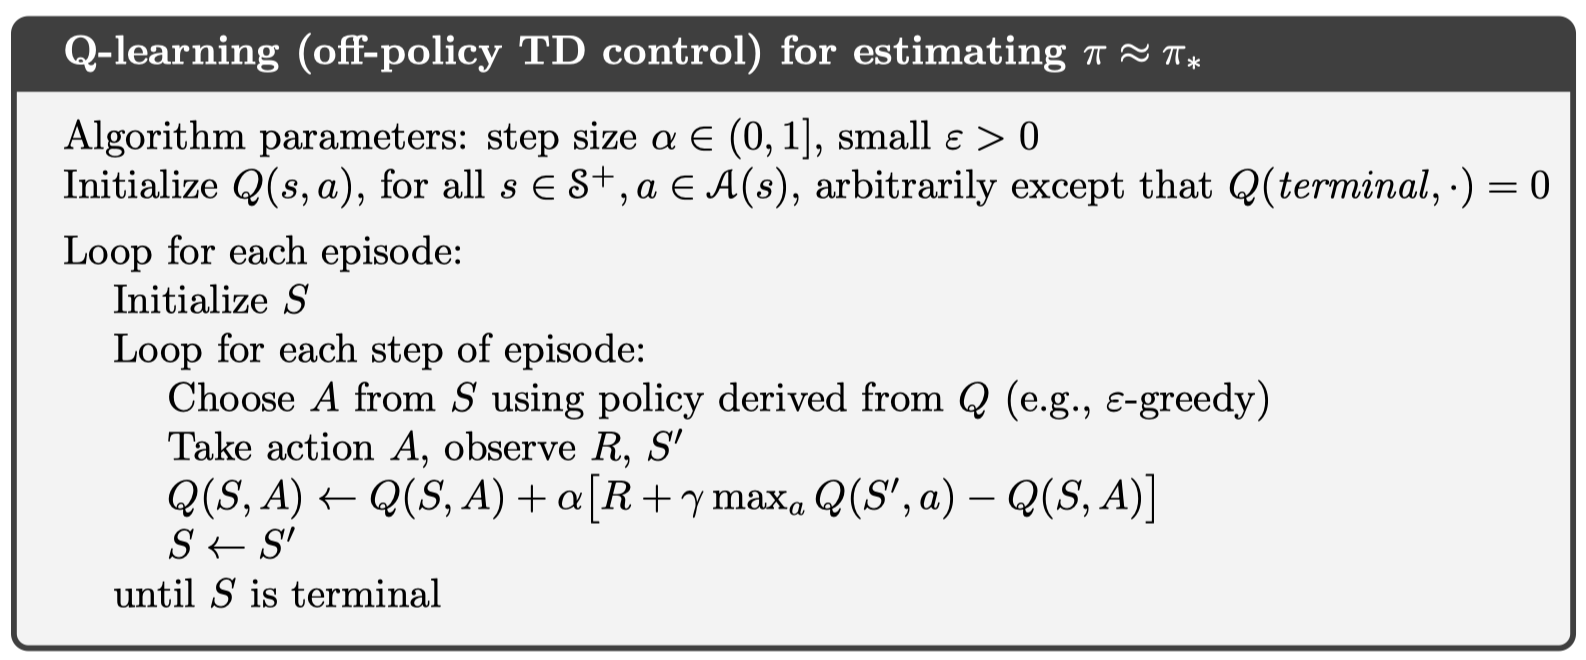
\includegraphics[width=0.7\textwidth]{image-2.png}
\end{figure}

We implement the above algorithm and we note that this is different from
SARSA where by the agent will always take the action that gives the maximum
reward. This is because the agent is not looking at the next state but the
maximum reward it can get from the next state.

\begin{lstlisting}[language=Python, caption=Qlearning code]
s = self.grid.state
action = self.get_action()
s_prime, reward = self.grid.next_step_and_reward(action)
self.quality[(s,action)] += \
        self.alpha * (
            reward + \
            self.gamma *
            max([self.quality[(s_prime,a)] for a in self.grid.action])\
            - self.quality[(s,action)]
        )
\end{lstlisting}

\section*{Results}

\begin{figure}[h]
    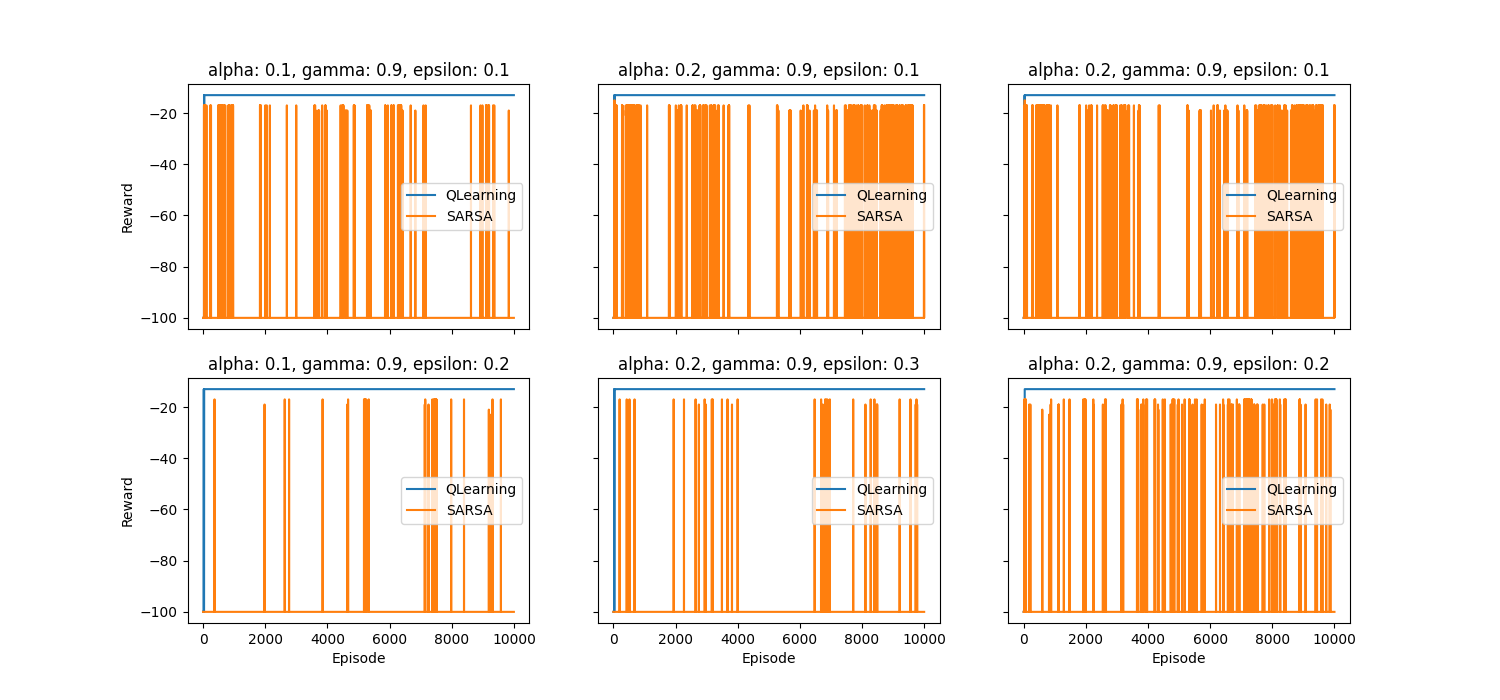
\includegraphics[width=15cm]{image-3.png}
    \caption{Performance of models based on different parameters}
\end{figure}

We can see that the Q learning algorithm has a higher average reward than the
SARSA algorithm. For different paramters, we can see that the Q learning
quickly converges to the optimal path while the SARSA algorithm takes a more
conservative approach. We also note that the SARSA algorithm reaches a state
where by the optimal path perceived is the safest path. This is the route that
is the furthest alway from the cliff. This is interesting as for different
parameters, especially with higher epsilon values, the agent should be exploring
but it still takes the safest path.

\begin{figure}[h]
    \centering
    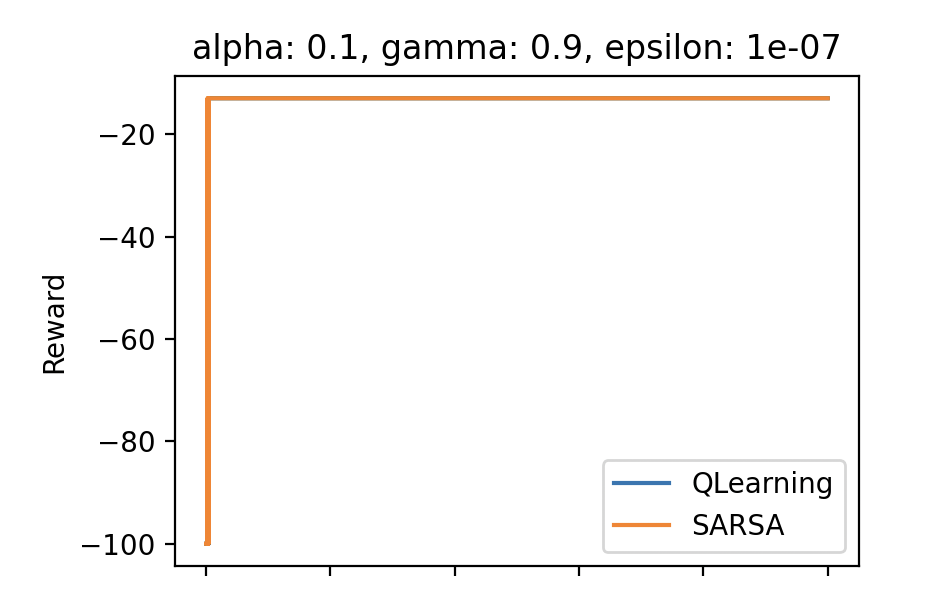
\includegraphics[width=0.7\textwidth]{image-4.png}
    \caption{Parameters to achieve optimal path}
\end{figure}

If we however, decrease the epsilon then both methods would asymptotically
converge to the optimal path. This is because the agent is not exploring and
taking the optimal path.

\section*{Conclusion}

From our SARSA algorithm, we can see that the agent always takes a more
conservative apporach through a one step look ahead. This allows

While Q learning algorithm is more aggressive in its approach. Instead of
looking one step ahead, it looks at the maximum reward it can get from the
next state. This allows the agent to take more risks and explore the gridworld.
Thus, we can see that when the agents reach their steady states, the Q learning
algorithm has a higher average reward than the SARSA algorithm (less negative).

However, as we saw, with a sufficiently low epsilon, both algorithms will
converge to the optimal path. This indicates that a low exploration but extreme
greedy approach will force the agent to take the optimal path..

\end{document}